% Don't touch this %%%%%%%%%%%%%%%%%%%%%%%%%%%%%%%%%%%%%%%%%%%
\documentclass[addpoints]{exam}
\usepackage{fullpage}
\usepackage[left=1.0in,top=1.0in,right=1.0in,bottom=1.0in,headheight=3ex,headsep=3ex]{geometry}
\usepackage{graphicx}
\usepackage{float}
\usepackage{adjustbox}
\usepackage{comment}
\usepackage{tikz}
\usetikzlibrary{calc}
\usetikzlibrary{matrix}
\usetikzlibrary{positioning}
\usepackage{amsmath}

\tikzset{   
	every picture/.style={remember picture,baseline},
	every node/.style={anchor=base,align=center,outer sep=1.5pt},
	every path/.style={thick},
}
\newcommand\marktopleft[1]{%
	\tikz[overlay,remember picture] 
	\node (marker-#1-a) at (-.3em,.3em) {};%
}
\newcommand\markbottomright[2]{%
	\tikz[overlay,remember picture] 
	\node (marker-#1-b) at (0em,0em) {};%
}
\tikzstyle{every picture}+=[remember picture] 
\tikzstyle{mybox} =[draw=black, very thick, rectangle, inner sep=10pt, inner ysep=20pt]
\tikzstyle{fancytitle} =[draw=black,fill=red, text=white]


\usepackage{graphicx,stackengine,xcolor}
\newcommand\Circle[1]{%
	\def\useanchorwidth{T}%
	\def\stacktype{L}%
	\stackon[0pt]{#1}{\scalebox{2.0}[1.15]{\textcolor{red}{$\bigcirc$}}}%
}
\newcommand{\blankline}{\quad\pagebreak[2]}
%%%%%%%%%%%%%%%%%%%%%%%%%%%%%%%%%%%%%%%%%%%%%%%%%%%%%%%%%%%%%%

% Modify Course title, instructor name, semester here %%%%%%%%

\title{ECN 453: Mid-term Exam 1: Practice}
% Modify header here %%%%%%%%%%%%%%%%%%%%%%%%%%%%%%%%%%%%%%%%%
\rhead{\footnotesize ECN 453: Mid-term Exam 1: Practice}

\date{} 

\begin{document}
	\maketitle
	\begin{center}
		\fbox{\fbox{\parbox{6in}{\centering\
					\textbf{Instructions}:
					\begin{itemize}
					\item You have \textbf{70 minutes}
					%\item Please write your final answer in the underlined section provided. 
					\item You may bring a calculator and notes on a two-sided cheat-sheet on letter-size paper. 
					\item Please be neat. If your work is too messy it will not be graded.
					\item Be sure to show your working.
					\item This is a long exam, so there are lots of ways to get points. If you get stuck, move on!
					\item Good luck!
					\end{itemize}	
			}}}
	\end{center}
	
	\vspace{5mm}
	\makebox[0.75\textwidth]{Name: \enspace\hrulefill}
	\vspace{50pt}
	\begin{center}
		\gradetable[h][questions]
	\end{center}
	
	\newpage
	
\begin{questions}
	\subsection*{1. Short Answer Questions (30 points)}
	\vspace{11pt}
	\question Depending on the question, write either: 
	\begin{itemize}
		\item a number 
		\item one of: True, False, or NEI (Not Enough Information)
		\item a definition (i.e. one or a few words)
	\end{itemize}
	\vspace{11pt}
	\begin{parts}
		\part[3] A monopolist faces a constant elasticity demand curve with elasticity -2 and has a constant marginal cost = 5. What is the optimal price?
		
		\answerline[answer]
		
		\part[3] Name one policy solution to monopoly power.
		
		\answerline[answer]
		
		\part[3] Name a second policy solution to monopoly power (different from your above answer).
		
		\answerline[answer]
		
		\part[3] True, False, or Not Enough Information: given two markets, a monopolist will always charge a higher \textit{price} in a market with more inelastic demand.
				
		\answerline[answer]
		
		\part[3] True, False, or Not Enough Information: there is a unique Nash equilibrium in every simultaneous game.
		
		\answerline[answer]
		
		\part[3] True, False, or Not Enough Information: there is no dead-weight-loss under perfect price discrimination.
		
		\answerline[answer]
		
		\part[3] Suppose that a monopolist has the cost $C(q)= 10+5q^2$ and the perfect competition price and quantity is at $p_{pc} = 10, q_{pc} = 1$. What subsidy will the regulator need to provide the monopolist to ensure it does not shutdown under \textit{marginal cost pricing}?

		\answerline[answer]
		
		\part[3] True, False, or Not Enough Information: consumers are always worse-off under price discrimination.
		
		\answerline[answer]
		
		\part[3]  True, False, or Not Enough Information: if there is a dominant strategy in a simultaneous game with two strategies and two players, then there is also a dominated strategy.
		
		\answerline[answer]
				
		\part[3] True, False, or Not Enough Information: suppose that there are two strategies $A$ and $B$ in a simultaneous game, and two players. If player 1 has a best response to $B$ of $A$, then player 2 has a best response of $B$ to $A$ as well.
		\answerline[answer]

	\end{parts}
	
	\begin{comment}
	\subsection*{Bertrand and Cournot Competition}
		\question There are three firms in a market and total demand is $p=120-2Q$. Firm 1 and Firm 2 have the same marginal cost and $c_1=c_2=10$. Firm 3 has the marginal cost $c_3=15$.
		\vspace{11pt}
	\begin{parts}
		\part[10] Suppose that the firms compete on prices (Bertrand Competition). What is the equilibrium total quantity?
		\part[15] Suppose that the firms compete on quantities (Cournot Competition). What is the equilibrium total quantity?
	\end{parts}

	\subsection*{Stackelberg/Entry Deterrence}
	\question There are two firms in a market with total demand $p=100-2Q$. Firm 1 is an incumbent and Firm 2 is a potential entrant. Firm 1's total cost is $C(q_1)=5q_1$.  Firm 2's total cost is $C(q_2)=10q_2^2$. The timing is as follows:
	\begin{enumerate}
		\item Firm 1 chooses $q_1$
		\item Firm 2 chooses whether to enter given $q_1$. If Firm 2 enters it pays an entry cost of $E \geq 0$.
		\item If Firm 2 enters then Firm 2 chooses $q_2$. 
	\end{enumerate}
	\vspace{11pt}
\begin{parts}
	\part[10] Suppose that $E=0$ and so Firm 2 will choose to enter. What are the equilibrium quantities for Firm 1 and Firm 2?
	\part[15] Suppose that $E=16$. Which values of $q_1$ deter Firm 2's entry?
	\part[5] Assume that $E=50$. What is the optimal $q_1$ for Firm 1?
\end{parts}

	
\item Assume that you cannot distinguish between students and non-students, and so you can only set a single \textit{uniform price} for all consumers.
\begin{enumerate}
\item (4 points) What is the total demand for movie seats under uniform pricing?
\item (4 points) What is the marginal revenue for movie seats under uniform pricing?
\item (8 points) What is the optimal uniform price? (Hint: plot marginal revenue.)
\item (2 points) What is the consumer surplus under uniform pricing?
%\item (2 points) What is the profit under uniform pricing?
\end{enumerate}
\item Assume that you \underline{can} distinguish between students and non-students, and so you can do \textit{price discrimination by indicators}.
\begin{enumerate}
\item (4 points) What are the optimal prices for students and non-students?
\item (2 points) What is the consumer surplus?
\end{enumerate}
\item (6 points) Suppose that there are only (identical) students in the market, and that the interpretation of the demand curve for students is now \textit{how many} tickets each student demands. What is the optimal two-part-tariff for students?

	\end{comment}
	
\subsection*{2. Price discrimination by indicators (30 points)}
	\question Suppose you are the owner of a movie theater. Assume that the marginal cost of a seat is \$20. There are two types of customers: students (denoted `s') and non-students (denoted `ns'). You know if a customer is a student or non-student and so you could potentially use price discrimination with \textit{selection by indicators}. The demand for movie seats for each of these segments is:
	\begin{align*}
		\text{Student: } &q_{s} = 50 - p_{s} \\
		\text{Non-student: }& q_{ns} = 100 - p_{ns}
	\end{align*}
	
	1. Assume that you cannot distinguish between students and non-students, and so you can only set a single \textit{uniform price} for all consumers.
	\begin{parts}
		\part[4] What is the total demand for movie seats under uniform pricing?
		\part[4] What is the marginal revenue for movie seats under uniform pricing?
		\part[8] What is the optimal uniform price? (Hint: plot marginal revenue.)
		\part[2] What is the consumer surplus under uniform pricing?
	\end{parts}
	\vspace{11pt}
    2. Assume that you \underline{can} distinguish between students and non-students, and so you can do \textit{price discrimination by indicators}.
    \begin{parts}
    	\part[4] What are the optimal prices for students and non-students?
    	\part[2] What is the consumer surplus?
    \end{parts}
	\vspace{11pt}
	3. Suppose that there are only (identical) students in the market, and that the interpretation of the demand curve for students is now \textit{how many} tickets each student demands. 
	\begin{parts}
		\part[6] What is the optimal two-part-tariff for students?
	\end{parts}
	
	\subsection*{3. Pricing airline tickets (30 points)}
	\question Suppose you are the CEO of an airline and there are two segments of airline ticket consumers: business and tourists. \underline{Marginal cost = \$30 per seat.} 
	
	There are two types of tickets: standard and restricted, where a restricted ticket has limitations about when/where it can be used (and so we can think of it as a `damaged' good). The number of consumers and willingness-to-pay for each consumer is given in the following table:
	
	\begin{centering}
		\begin{table}[h]
			\centering
			\begin{tabular}{|l|c|c|c|}
				\hline
				\textbf{Consumer type}&  \textbf{Number of consumers} & \multicolumn{2}{c}{\textbf{Willingness to pay (\$)}} \\
				%\hline
				& & Standard & Restricted  \\
				\hline
				Business & 10 & 180 & 80  \\
				\hline
				Tourist & 30  & 60 & 50  \\
				\hline
			\end{tabular}
		\end{table}
	\end{centering}
	\vspace{11pt}
	1. Assume that you \underline{can} distinguish between business and tourist consumers.
	\begin{parts}
		\part[5] What is the profit under perfect price discrimination?
	\end{parts}
	\vspace{11pt}
	2.  Assume that you cannot distinguish between business and tourist consumers.
	\begin{parts}
		\part[5] If you can only offer the standard ticket, what is the optimal uniform price?
		\part[5] Suppose that you charge $\$180$ for the standard ticket and $\$50$ for the restricted ticket. What is the airline's profit?
		\part[5] Suppose that you charge $\$90$ for the restricted ticket. What is the optimal price for the standard ticket?
		\part[10]Suppose that you charge $\$50$ for the restricted ticket. What is the optimal price for the standard ticket?
	\end{parts}
	
	\subsection*{4. Game theory (30 points)}
	\question
	Consider the following game (where `x' stands for a number).
	
	\begin{figure}[h]
		\centering
		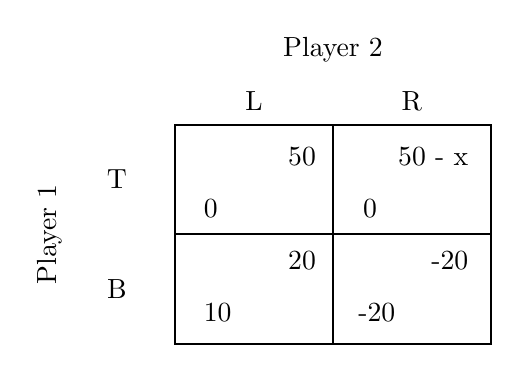
\begin{tikzpicture}
			\matrix[matrix of math nodes,every odd row/.style={align=right},every evenrow/.style={align=left},every node/.style={text width=1.5cm},row sep=0.2cm,column sep=0.2cm,ampersand replacement=\&] (m) {
				50 \& 50 - x \\
				0 \phantom{---------} \& 0 \phantom{--------} \\
				20 \& -20\\
				10 \phantom{--------} \& -20 \phantom{------}  \\
			};
			\draw (m.north east) rectangle (m.south west);
			\draw (m.north) -- (m.south);
			\draw (m.east) -- (m.west);
			
			% Player 1
			\coordinate (c) at ($(m.north west)!0.25!(m.south west)$);
			\coordinate (d) at ($(m.north west)!0.75!(m.south west)$);
			\node[left=2pt of c,text width=1cm]  {T};
			\node[left=2pt of d,text width=1cm]  {B};
			
			% Player 2
			\coordinate (a) at ($(m.north west)!0.25!(m.north east)$);
			\coordinate (b) at ($(m.north west)!0.75!(m.north east)$);
			\node[above=5pt of a,anchor=base] {L};
			\node[above=5pt of b,anchor=base] {R};
			
			\node[above=18pt of m.north] (firm b) {Player 2};
			\node[left=1.6cm of m.west,rotate=90,align=center,anchor=center] {Player 1};
			
			%\node[above=5pt of firm b]  {Payoff Matrix};
		\end{tikzpicture}
	\end{figure}
	
	\begin{parts}
		\part[5] Assume that $x=0$. What are all the Nash equilibria?
		\part[5]  Provide a value of $x$ where (B,L) is the \textit{unique} Nash equilibrium?
		\part[10]  Assume that $x=0$ and that the players play (B,L) in the simultaneous game. How much would player 2 pay to commit to moving first? (Hint: it might be helpful to write out the sequential game.)
		\part[10] Assume that player 2 moves first. Provide a value of $x$ to ensure that $(B,L)$ is the unique subgame-perfect equilibrium.
	\end{parts}
\end{questions}


\end{document}